\chapter*{Introduzione}

L'industria dello sviluppo di videogiochi ha raggiunto negli ultimi anni livelli di complessità tecnica e fedeltà visiva senza precedenti. In questo contesto, l'utilizzo di motori grafici avanzati come Unity permette di realizzare scenari fotorealistici, ma pone sfide significative in termini di efficienza computazionale e gestione delle risorse hardware.

\begin{figure}[htbp]
    \centering
    \begin{minipage}{0.48\textwidth}
        \centering
        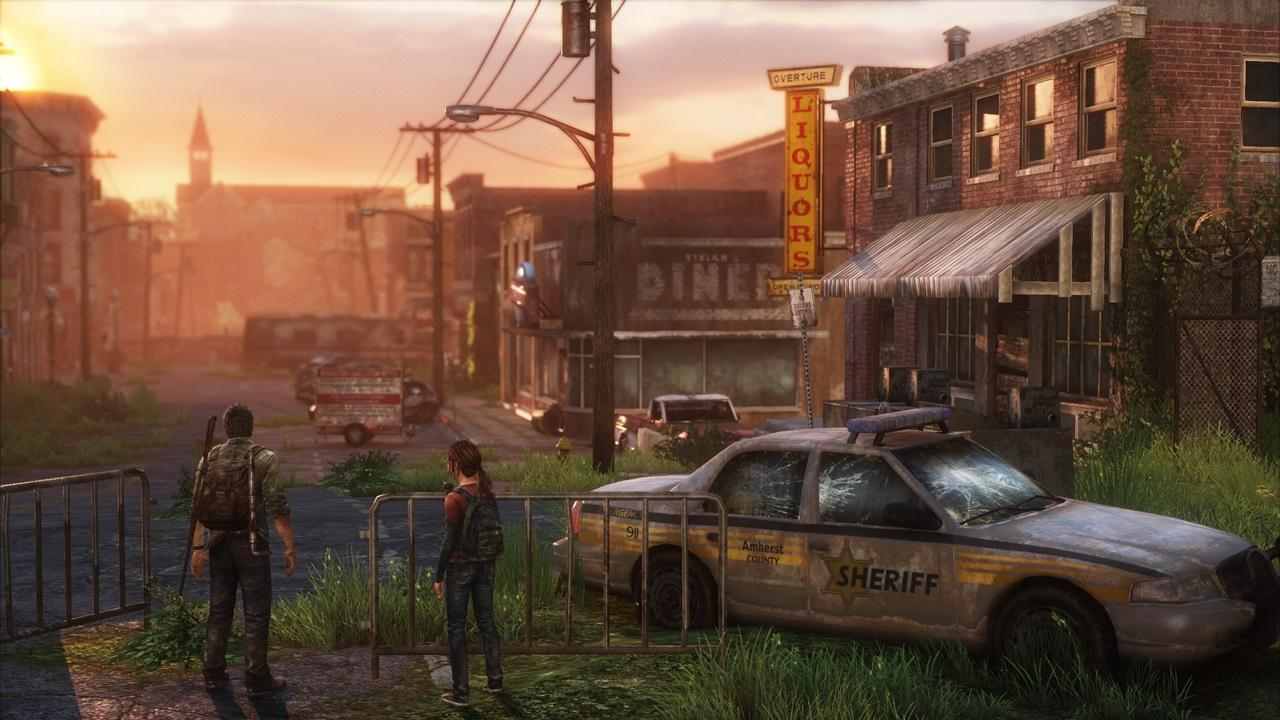
\includegraphics[width=\textwidth]{immagini/lastofus.jpg}
        \caption*{\small The Last Of Us.}
    \end{minipage}
    \hfill % Spazio flessibile tra le due immagini
    \begin{minipage}{0.48\textwidth}
        \centering
        
\includegraphics[width=\textwidth]{immagini/rdr2.jpg}
        \caption*{\small Red Dead Redemption II}
    \end{minipage}
\end{figure}

Il progetto, denominato ARES, consiste in un videogioco sviluppato tramite la High Definition Rendering Pipeline (HDRP) di Unity, una tecnologia progettata per massimizzare la resa grafica a fronte di un elevato carico sulla GPU. L'obiettivo principale della sperimentazione è stato l'analisi e l'ottimizzazione delle performance di rendering del titolo. In particolare, l'attenzione si è focalizzata sulla riduzione delle \textit{draw call}, sulla gestione dei \textit{batch} e sullo sviluppo di shader personalizzati volti a migliorare il frame rate senza compromettere la qualità estetica.